%************************************************
\chapter{RAFFT: Efficient prediction of fast-folding pathways of RNAs}\label{ch:rafft}
%************************************************
This chapter introduces a novel heuristic algorithm to predict an ensemble of metastable \ac{RNA} secondary structures for a given sequence $\phi$. The algorithm is inspired by the kinetic partitioning mechanism, by which molecules follow alternative folding pathways to their native structure, some much faster than others. Similarly, our algorithm \texttt{RAFFT} generates an ensemble of concurrent folding pathways ending in multiple metastable structures for each given sequence. We then use the ensemble structures as finite ensemble states in which the \ac{RNA} sequence can be at a given time, and the energy difference from one state to another is then used to derive a stem rate model. Therefore, our algorithm also acts as a folding kinetic ansatz. Much of the material in this chapter has been previously described in \cite{opuu2021rafft}.
\section{Material and Methods}
The computational time is one of the challenges for the existing tool in folding long \ac{RNA} molecules. The method we present in this work aims to improve the existing \ac{RNA} folding tools reviewed in \autoref{ch:folding}. It is based on the \ac{FFT} and inspired by the kinetic partitioning mechanism. As presented in \autoref{ch:introduction}, the \ac{FFT} allows reducing the computational time of the correlation between two sequences. We use the same ideal in the context of this work to faster predict \ac{RNA} folding pathways by analyzing high correlation positional lag between an \ac{RNA} sequence and its complementary copy, especially for longer sequences. We, therefore, derive a kinetics ansatz from the structural ensemble of the predicted folding paths. 
This section describes our \ac{RNA} pathways prediction method and the kinetics ansatz derived from the predicted structural ensemble. In addition, it provides a description of the benchmark dataset used to assess our method performance and the comparison protocols. 
\subsection{\texttt{RAFFT}'s  algorithm description}
\texttt{RAFFT} starts from a sequence of nucleotides \(\phi=(\phi_1\dots \phi_L)\) of length \(L\), and its associated unfolded structure $\sigma$. We first create a numerical representation of \(\phi\) where each nucleotide is replaced by a unit vector of $4$ components:
\begin{equation}
\begin{split}
\text{A} \rightarrow \begin{pmatrix} 1\\ 0\\ 0\\ 0 \end{pmatrix},
\text{U} \rightarrow \begin{pmatrix} 0\\ 0\\ 0\\ 1 \end{pmatrix},
\text{C} \rightarrow \begin{pmatrix} 0\\ 1\\ 0\\ 0 \end{pmatrix},
\text{G} \rightarrow \begin{pmatrix} 0\\ 0\\ 1\\ 0 \end{pmatrix}.
\end{split}
\end{equation}
This encoding gives us a (\(4 \times L\))-matrix we call \(X\), where each row corresponds to a nucleotide as shown below:
\begin{equation}
X = \begin{pmatrix} X^{\text{A}}\\ X^{\text{C}}\\ X^{\text{G}}\\ X^{\text{U}} \end{pmatrix} = \begin{pmatrix} X^{\text{A}}(1) &X^{\text{A}}(2) &\dots &X^{\text{A}}(L) \\ X^{\text{C}}(1) &X^{\text{C}}(2) &\dots &X^{\text{C}}(L)\\ X^{\text{G}}(1) &X^{\text{G}}(2) &\dots &X^{\text{G}}(L)\\ X^{\text{U}}(1) &X^{\text{U}}(2) &\dots &X^{\text{U}}(L) \end{pmatrix}.
\end{equation}
For example, \(X^{\text{A}}(i) = 1\) if \(\phi_i = \text{A}\). Next, we create a second copy \(\bar{\phi}=(\bar{\phi_L}\dots \bar{\phi_1})\) for which we reversed the sequence order. Then, each nucleotide of \(\bar{\phi}\) is replaced by one of the following unit vectors:
\begin{equation}
\begin{split}
\bar{\text{A}} \rightarrow \begin{pmatrix} 0\\ 0\\ 0\\ w_{\scalebox{0.5}{AU}}\\ \end{pmatrix},
\bar{\text{U}} \rightarrow \begin{pmatrix} w_{\scalebox{0.5}{AU}}\\ w_{\scalebox{0.5}{GU}}\\ 0\\ 0\\ \end{pmatrix},
\bar{\text{C}} \rightarrow \begin{pmatrix} 0\\ 0\\ w_{\scalebox{0.5}{GC}}\\ 0\\ \end{pmatrix},
\bar{\text{G}} \rightarrow \begin{pmatrix} 0\\ w_{\scalebox{0.5}{GC}}\\ 0\\ w_{\scalebox{0.5}{GU}}\\ \end{pmatrix}.
\end{split}
\end{equation}
\(\bar{\text{A}}\) (respectively \(\bar{\text{U}}, \bar{\text{U}}, \bar{\text{G}}\)) is the complementary of \(\text{A}\) (respectively \(\text{U}, \text{C}, \text{G}\)). \(w_{AU}\), \(w_{GC}\), \(w_{GU}\) represent the weights associated with each canonical base-pair, and they are chosen empirically. We call this complementary copy \(\bar{X}\), the mirror of \(X\).

To search for stems, we use the complementary relation between \(X\) and \(\bar{X}\) with the correlation function \(\text{cor}(k)\). This correlation is defined as the sum of individual \(X\) and \(\bar{X}\) row correlations
\begin{equation}
\text{cor}(k)=\sum_{\alpha \in \{\text{A},\text{U},\text{C},\text{G}\}}c_{X^{\alpha},\bar{X}^{\alpha}}(k)
\end{equation}
where a row correlation between \(X\) and \(\bar{X}\) is given by
\begin{equation}
c_{X^\alpha,\bar{X}^\alpha}(k) = \sum\limits_{\substack{1\leq i \leq L\\1 \leq i + k \leq L}} \frac{X^\alpha(i) \bar{X}^\alpha(i+k)}{\text{min}(k, 2 L-k)}.
\end{equation}
For each \(\alpha \in \{\text{A},\text{U},\text{C},\text{G}\}\), \(X^\alpha(i) \times \bar{X}^\alpha(i+k)\) is non zero if sites \(i\) and \(i+k\) can form a base-pair, and will have the value of the chosen weight as described above. If all the weights are set to $1$, \(\text{cor}(k)\) gives the frequency of base-pairs for a positional lag \(k\). Although the correlation naively requires \(O(L^2)\) operations, it can take advantage of the \ac{FFT} which reduces its complexity to \(\mathcal{O}(L\;\text{log}(L))\).

Large \(\text{cor}(k)\) values between the two copies indicate positional lags \(k\) where the frequency of base-pairs is likely to be high. However, this does not allow to determine the exact stem positions. Hence, we use a sliding window strategy to search for the largest stem within the positional lag (since the copies are symmetrical, we only need to slide over one-half of the positional lag). Once the largest stem is identified, we compute the free energy change associated with the formation of that stem. Next, we perform the same search for the \(n\) highest correlation values, which gives us \(n\) potential stems. Then, we define as the current structure the stem with the lowest free energy. Here, free energies were computed using Turner2004 energy parameters through ViennaRNA package \ac{API} \cite{lorenz11_vienn_packag}.


\begin{figure*}[t!]
	\centering
	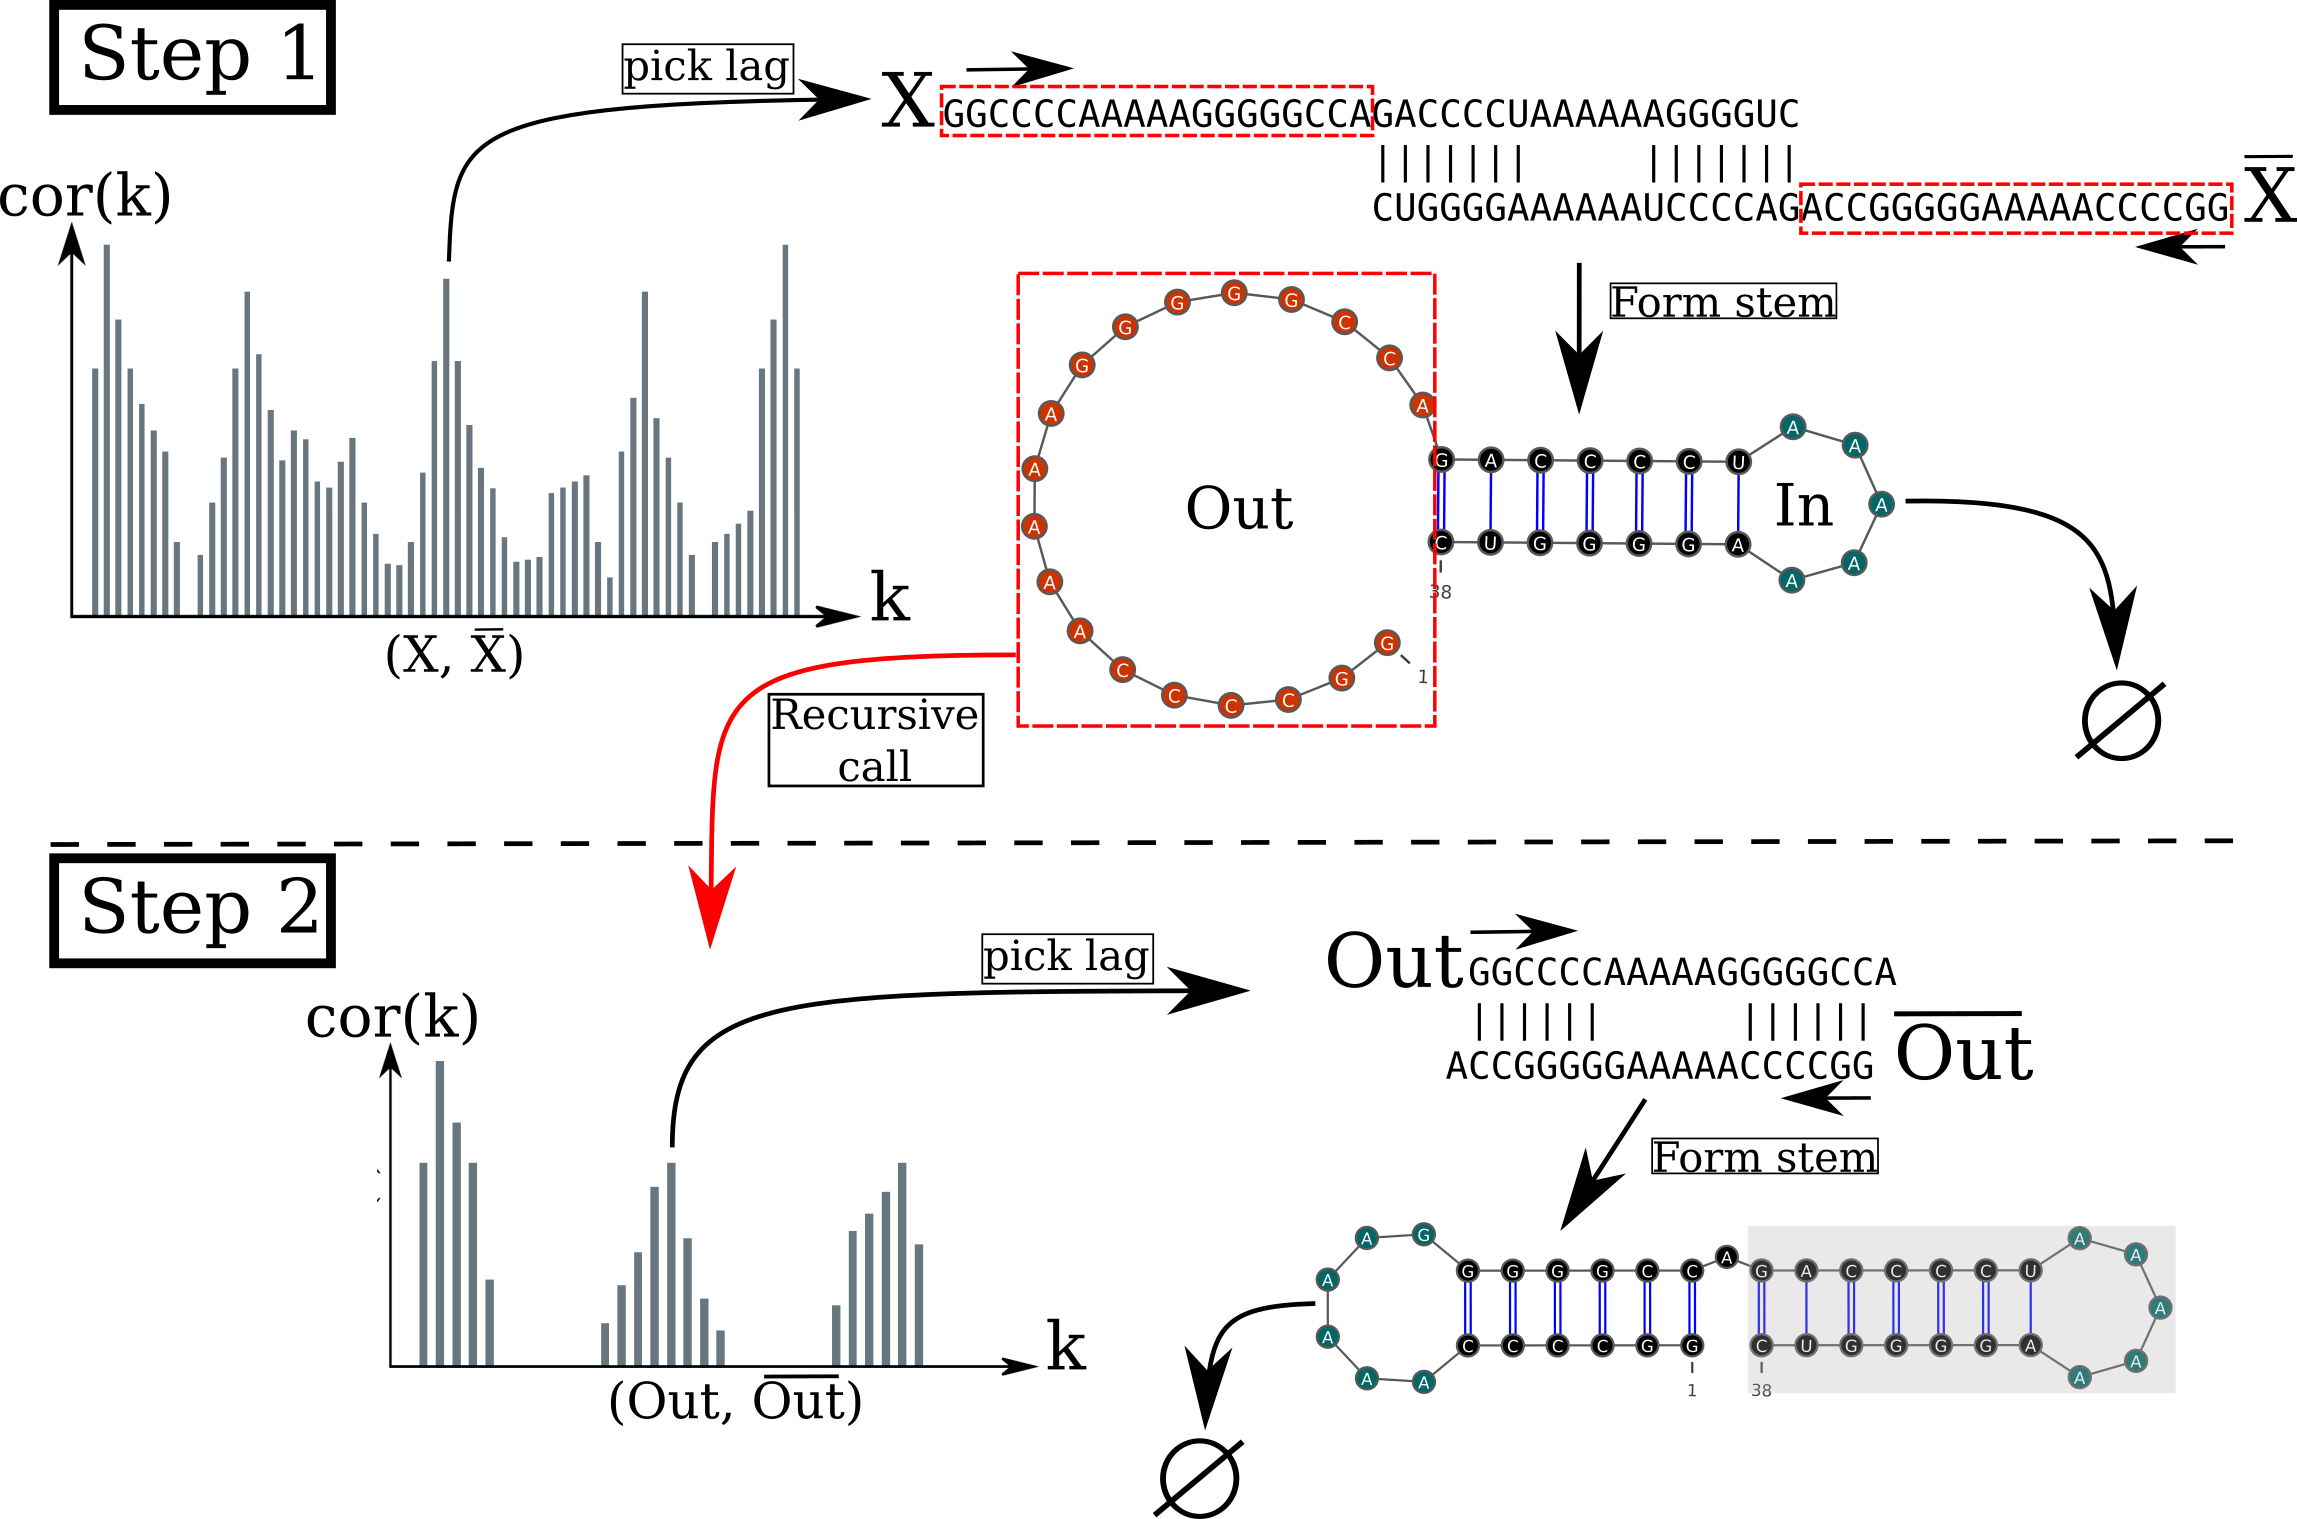
\includegraphics[width=1.\linewidth]{../res/images/rafft/algo_draw.png}
	\caption{\label{algo_desc}\textbf{Algorithm execution for one example sequence which requires two steps.} (Step 1) From the correlation $cor(k)$, we select one peak which corresponds to a position lag $k$. Then, we search for the largest stem and form it. Two fragments, ``In" (the interior part of the stem) and ``Out" (the exterior part of the stem), are left, but only the ``Out" may contain a new stem to add. (Step 2) The procedure is called recursively on the ``Out" sequence fragment only. The correlation $cor(k)$ between the ``Out'' fragment and its mirror is then computed and analyzing the $k$ positional lags allows to form a new stem. Finally, no more stem can be formed on the fragment left (colored in blue), so the procedure stops.}
\end{figure*}

We are now left with two independent parts, the interior and the exterior of the newly formed stem. If the exterior part is composed of two fragments, they are concatenated into one. Then, we apply recursively the same procedure on the two parts independently in a \textit{breadth-first} fashion to form new consecutive base-pairs. The procedure stops when no base-pair formation can improve the energy. When multiple stems can be formed in these independent fragments, we combine all of them and pick the composition with the best overall stability. If too many compositions can be formed, we restrict this to the $10^4$ bests in terms of energy. \autoref{algo_desc} shows an example of execution to illustrate the procedure. 
\begin{figure}[t!]
	\centering
	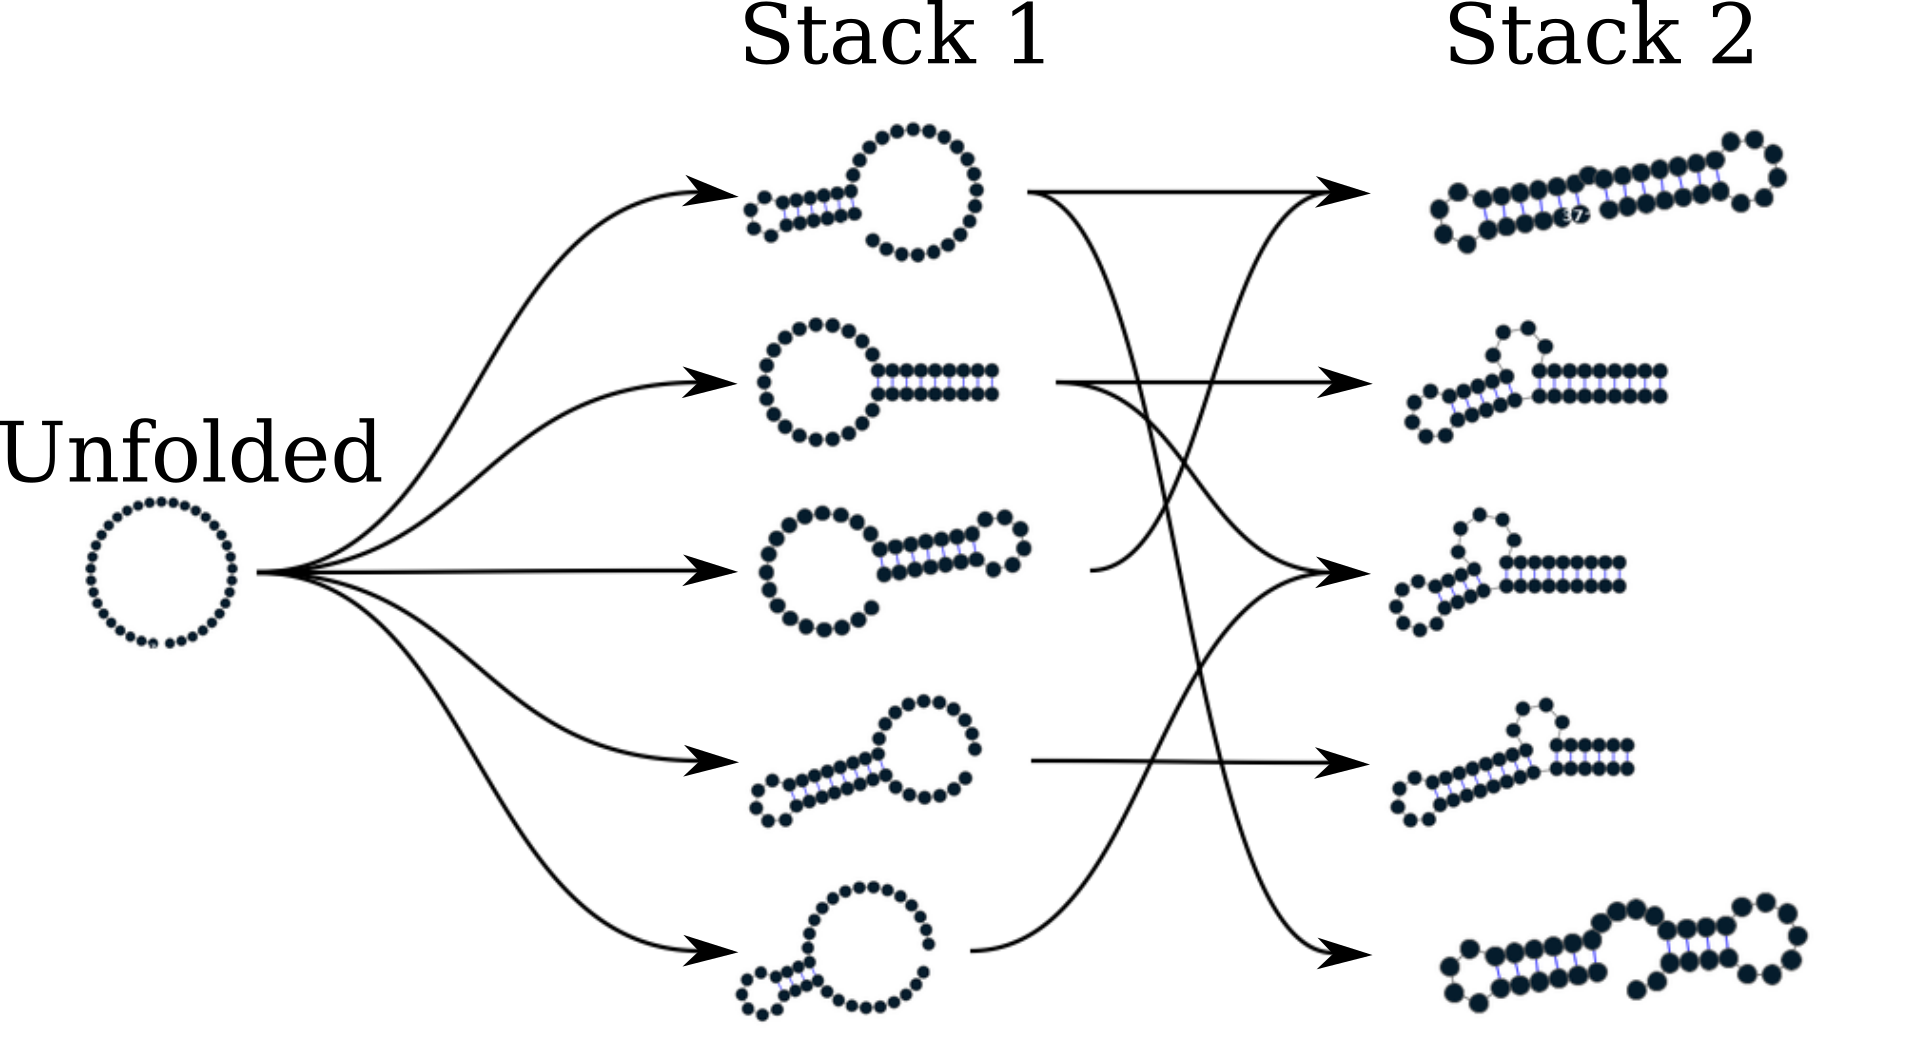
\includegraphics[width=1\linewidth]{../res/images/rafft/fast_paths_graph.png}
	\caption{\label{fast_path_graph}\textbf{Fast folding graph constructed using \texttt{RAFFT}.} In this example, the sequence is folded in two steps. The algorithm starts with the unfolded structure on the left. The \(N=5\) best stems are stored in stack 1. From stack 1, multiple stems formation are considered, but only the \(N=5\) best are stored in stack 2. Structures are ordered (from top to bottom) by energy in each stack. All secondary structure visualizations were obtained using \texttt{VARNA} \cite{darty09_varna}.}
\end{figure}

The algorithm described so far tends to be stuck in the first local minima found along the folding trajectory. To alleviate this, we implemented a stacking procedure where the \(N\) best trajectories are stored in a stack and evolved in parallel. Like the initial version, the algorithm starts with the unfolded structure; then, the \(N\) best potential stems are stored in the first stack. From these \(N\) structures, the procedure tries to add stems in the unpaired regions left and saves the \(N\) best structures formed. Once no stem can be formed, the algorithm stops and output the structure with the best energy found among the structures stored in the last stack. This algorithm leads to the construction of a graph we call a \emph{fast-folding graph}. In this graph, two structures are connected if the transition from one to another corresponds to the formation of a stem or if the two structures are identical. \autoref{fast_path_graph} shows an example of a \emph{fast-folding graph} produced by \texttt{RAFFT} for $N=5$.

This section presented the complete procedure implemented in our proposed tool \texttt{RAFFT}. The procedure resulted in an ensemble of concurrent folding pathways ending in multiple metastable secondary structures. The connections in each folding pathway are dictated by the formation of stems, resulting in an energy increase. The different folding pathways connected to the initial unfolded structure form a fast folding graph. The ensemble of secondary structures constituting the fast folding graph is then used to build our kinetics ansatz where the transitions follow the Metropolis rules, i.e. no barriers between structures. The following section provides more details on our proposed kinetics ansatz.
\subsection{Kinetic ansatz}
Now that the RNA pathway prediction algorithm is described, we provide the ingredients needed to extract dynamic folding information from the previously generated fast folding graph in this section.

The folding kinetic ansatz used here is derived from the fast-folding graph and allows us to model the slow processes in \ac{RNA} folding. As described in \autoref{fast_path_graph}, transitions can occur from left to right (and right to left) but not vertically. The fast-folding graph follows the idea that parallel pathways quickly reach their endpoints; however, when the endpoints are non-native states, this ansatz allows slowly folding back into the native state \cite{pan97_foldin_rna_invol_paral_pathw}. 

Using the master-equation (See \autoref{Eq:kenetics}), the traditional kinetic approach often starts by enumerating the whole space (or a carefully chosen subspace) of structures using \texttt{RNAsubopt}. Next, this ensemble is divided into local attraction basins separated from one another by energy barriers. This coarsening is usually done with the tool called \texttt{barriers}. Then, following the Arrhenius formulation (See \autoref{Eq:arrhenius}) , one simulates a coarse grained kinetics between basins.  

In contrast to traditional kinetics approaches, the connected structures in the \texttt{RAFFT}'s fast-folding graph are not always separated by activation barrier energies. Therefore, we computed the transition rates $k_{i\rightarrow j}$ using the Metropolis \cite{klemm2008funnels} formulation defined as
\begin{equation}
\label{Eq:metropolis}
k_{i\rightarrow j} = \begin{cases}
k_0 \times \text{min}(1, \text{exp}(-\beta \Delta (\Delta G_{i \rightarrow j}))),& \text{if } \sigma_i \in \mathcal{M}(\sigma_j) \\
0,& \text{else }
\end{cases}
\end{equation}
where \(\Delta \Delta G_{i\rightarrow j} = \Delta G_j - \Delta G_i\) is the free energy change between structure \(\sigma_i\) and \(\sigma_j\). Here, \(k_0\) is a conversion constant that we set to $1$ for the sake of simplicity and we initialize the population \(p_i(0)\) with only unfolded structures; therefore, the trajectory represents a complete folding process. The frequency of a structure \(\sigma_i\) evolves according to the master \autoref{Eq:kenetics}. Due to this approximation, we referred to our approach as a \textit{kinetic ansatz}

In sum, based on the \ac{FFT}, we constructed a method that allows generating an ensemble of secondary structures by a successive formation of stems. Using this ensemble, we derived a kinetics ansatz in which transitions between structures follow the Metropolis rules. We assess the performance of our tool by comparing its predictions to existing tools using benchmark datasets. The following section briefly describes the datasets used in this work, including the clean procedure applied to the initial datasets.

\subsection{Benchmark datasets. }

Measuring the performance of computational RNA folding tools can be quite a challenging task. A perfect validation procedure will require a comparison to experimental data, which in practice are not also perfect and are very expensive. In the context of this work, we perform \textit{in silico} validation using benchmark datasets, which is a collection of native sequence structures. Because our proposed method produces kinetics and static structure predictions., we assess the performance of both tasks separately and using a different dataset. This section presents the two datasets.

To build the dataset for the folding task application, we started from the \texttt{ArchiveII} dataset derived from multiple sources \cite{andronescu08_rna_stran,brown98_ribon_p_datab,bellaousov10_probk,daub08_rna_wikip,damberger94_compar_datab_group_i_intron_struc,zwieb00_tmrdb,zwieb03_tmrdb,waring84_asses_model_intron_rna_secon,specht97_compil_rrna_rrna_gene_sequen,sprinzl98_compil_trna_sequen_sequen_trna_genes,sloma16_exact_calcul_loop_format_probab,schnare96_compr_compar_struc_charac_eukar,mathews99_expan_sequen_depen_therm_param,samuelsson99_signal_recog_partic_datab_srpdb,gutell93_compil_large_subun_like_ribos_rna_struc,gutell94_collec_small_subun_like_ribos_rna_struc,gardner09_rfam}. We first removed all the structures with pseudoknots, since the tools considered here do not handle these loops. Next, using the Turner2004 energy parameters, we evaluated the structures' energies and removed all the unstable structures: structures with energies $\Delta G > 0$. This dataset is composed of $2,698$ sequences with their corresponding known structures. $240$ sequences were found multiple times (from $2$ to $8$ times); $19$ of them were mapped to different structures. For the sequences that appeared with different structures, we picked the structure with the lowest energy. In the end we arrived at a dataset with $2,296$ sequences-structures.

For the kinetics task, there is no existing standard procedure or dataset allowing to validate or not a computational tool. However, for the validation of our kinetic ansatz, we used the \ac{CFSE} \ac{RNA} sequence and classic bi-stable sequence \textbf{GGCCCCUUUGGGGGCCAGACCCCUAAAGGGGUC}. 
%The \ac{CFSE} \ac{RNA} sequence was taken from \texttt{RFAM}

In sum, two different dataset sets are used to assess \texttt{RAFFT} performance: the first one,  \texttt{Archive II}  consists of $2,296$ sequences-structures used for the prediction task, and one which contains two sequences, the CFSE and a bistable sequence for the kinetic study. The following section describes the benchmarking protocols for both tasks. 

\subsection{Structure prediction protocols}
The static RNA structure prediction and the  RNA kinetic performances of our proposed tool \texttt{RAFFT} are evaluated separately. This section describes the evaluation protocols for both performances and the different tool parameters used throughout.

To evaluate the structure prediction accuracy of the proposed method, we compared \texttt{RAFFT} to five recent secondary structure pseudoknot-free prediction tools. The five tools include \ac{ML}-based methods (\texttt{Mxfold2 0.1.1} and \texttt{Contrafold}) and score-based methods ( \texttt{RNAfold 2.4.13},  \texttt{Linearfold},  and \texttt{RNAstructure} ). To compute the \ac{MFE} structure for the score-based methods, we used the default parameters and the Turner2004 set of energy parameters. We also computed the \ac{ML} predictions using the default parameters. Therefore, only one structure prediction per sequence for these tools was used for the statistics.

Two parameters are critical for \texttt{RAFFT}, the number of positional lags in which stems are searched, and the number of structures stored in the stack. For our computational experiments, we searched for stems in the $n=100$ best positional lags and stored $N=50$ structures. The correlation function \(\text{cor}(k)\) which allows to choose the positional lags is computed using the weights \(w_{GC}=3\), \(w_{AU}=2\), and \(w_{GU}=1\).

To assess the performance of \texttt{RAFFT}, we analyzed the output in two different ways. First, we considered only the structure with the lowest energy found for each sequence. This procedure allows us to assess \texttt{RAFFT} performance in predicting the \ac{MFE} structure. Second, we computed the accuracy of all $N=50$ structures saved in the last stack for each sequence and displayed only the best structure in terms of accuracy. As mentioned previously in \autoref{ch:folding}, the lowest energy structure found may not be the active structure. Therefore, this second assessment procedure allows us to show whether one of the pathways is biologically relevant.

We used two metrics to measure the prediction accuracy: the \ac{PPV} and the sensitivity. The \ac{PPV} measures the fraction of correct base-pairs in the predicted structure, while the sensitivity measure the fraction of base-pairs in the accepted structure that are predicted. These metrics are defined in \autoref{ch:introduction} (See definitions \autoref{def:ppv}, \autoref{def:sensitivity}). 
To be consistent with previous studies, we computed these metrics using the \texttt{scorer} tool provided by Matthews \emph{et al.} \cite{mathews19_how_to_bench_rna_secon}, which also provides a more flexible estimate where shifts are allowed.

Further more, we used a \ac{PCA} to visualize the loop diversity in the predicted structures for each folding tool considered here. To extract the weights associated with each structure loop from the dataset, we first converted the structures into weighted coarse-grained tree representation \cite{shapiro1990comparing}. In the tree representation, the nodes are generally labelled as E (exterior loop), I (interior loop), H (hairpin), B (bulge), S (stacks or stem-loop), M (multi-loop) and R (root node). We separately extracted the corresponding weights for each node, and the weights are summed up and then normalized. Excluding the root node, we obtained a table of $6$ features and \(n\) entries. This allows us to compute a \(6\times 6\) correlation matrix that we diagonalize using the \texttt{eigen} routine implemented in the \texttt{scipy} package. For visual convenience, the structure compositions were projected onto the first two \acp{PC}. 

Finally, the \ac{CFSE} and a bistable \ac{RNA} sequence are used to assess the kinetic performance. For each sequence, initial conditions are chosen for both \texttt{Treekin} and \texttt{RAFFT} to simulate the kinetic trajectories. Both kinetics are simulated using the master equation described in \autoref{ch:folding} (\autoref{Eq:kenetics}) but with different transition rules, \texttt{Treekin} uses the Arrhenius rules whereas \texttt{RAFFT} uses the Metropolis rules. The following section describes the statistical results obtained for both kinetics and structure prediction tasks. 

\section{Experimental results }

The validation of our results is purely statistical, i.e. using statistical methods such as $t$-test and regression to compare different tool performance data. Based on the previously mentioned limitations of existing tools, we evaluate three main \texttt{RAFFT} potential improvements: the running time for the folding or pathways prediction, the quality of the predicted pathways and the \ac{RNA} folding kinetics. This section discusses each of those performances in comparison to the existing tools. 

\subsection{ \texttt{RAFFT}'s run time and scalability}

\begin{figure}[t!]
	\centering
	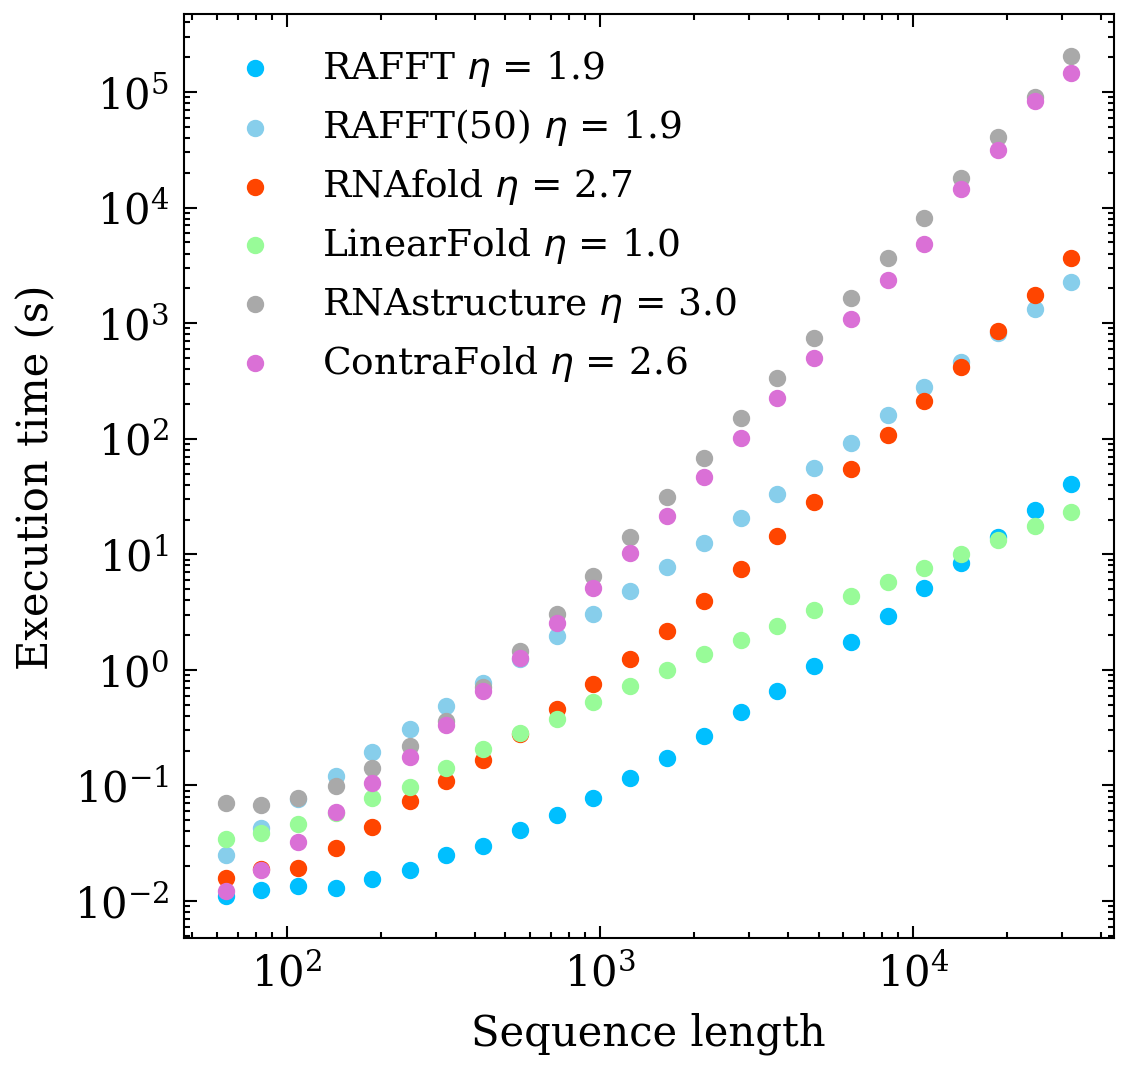
\includegraphics[width=1.0\linewidth]{../res/images/rafft/time_tools.png}
	\caption{\label{Fig:time_comp}\textbf{Execution time comparisons}. For samples of $30$ sequences per length, we averaged the execution times of five folding tools. The empirical time complexity $O(L^\eta)$ where $\eta$ is obtained by non-linear regression. \texttt{RAFFT} denotes the naive algorithm( with only $N=1$ structure saved per stack), whereas \texttt{RAFFT(50)} denotes the algorithm where $50$ structures can be saved per stack.}
\end{figure}
The first input of our method is a potential improvement to the \ac{CPU} time of existing tools. This section focuses on analyzing \texttt{RAFFT}'s running time compared to existing methods. Four different tools are considered: \texttt{RNAfold}, \texttt{ContraFold}, \texttt{RNAstructure}  and \texttt{LinearFold}. All of them are \texttt{MFE} estimates implementing a \texttt{DP} with cubic time complexity($O(L^3)$), except for \texttt{ContraFold} which implements a ML approach. When using the heuristic implementation of \texttt{LinearFold}, the time complexity is linear while losing the \texttt{MFE} estimation. We will first discuss \texttt{RAFFT} theoretical time complexity before comparing the empirical execution times to the existing tools.

The complexity of \texttt{RAFFT}'s algorithm depends on the number and size of the stems formed. The main operations performed for each stem formed are: (1) the evaluation of the correlation function \(\text{cor}(k)\), (2) the sliding-window search for stems, and (3) the energy evaluation. We based our approximate complexity on the correlation evaluation since it is the more computationally demanding step; the other operations only contribute a multiplicative constant at most. The best case is the trivial structure composed of one large stem where the algorithm stops after evaluating the correlation on the complete sequence. At the other extreme, the worst case is one where at most \(L/2\) stems of size $1$ (exactly one base-pair peer stems) can be formed. The approximate complexity therefore depends on 

\begin{equation}
\label{Eq:complexity}
\sum_{i=0}^{L/2} (L-2i) \log(L-2i) \ = O(L^2\log{L}).
\end{equation}

We compared \texttt{RAFFT}'s execution time to the classical cubic-time algorithms represented by \texttt{CONTRAfold} (Version 2.02), \texttt{RNAstructure} (Version 2.0), \texttt{RNAfold} (Version 2.4.13) and the recent improved \ac{DP} tool \texttt{LinearFold} (Version 1.0). \autoref{Fig:time_comp} shows the execution time of the \texttt{RUST} implementation of \texttt{RAFFT} and the four above-mentioned tools for $30$ random generated sequences of various lengths.  When comparing \texttt{RAFFT} implementation to the standard \ac{DP} tools, the execution time of \texttt{RAFFT} scales slower (with an exponent $\approx 2$) with the sequence length whereas the standard \ac{DP} execution times are cubic. In contrast, the execution time of the improved \ac{DP} implemented by \texttt{LinearFold} scales linearly with the sequence length. Only when considering a stack size of $1$, that \texttt{RAFFT} execution time is lower than the one of \texttt{LinearFold} for sequence of lengths less than $L=10^4$.

We also analyse the scalability of \texttt{RAFFT} computational time with respect to its critical parameters (the number  of positional lag $n$ and the stack size $N$). \autoref{Fig:scalability} shows for both different stack sizes and number of positional lags, \texttt{RAFFT} execution time against the sequence length. For both stack size and number of positional lags, the execution time scales almost with the same exponent ($\approx 2$).

\begin{figure}[t!]
	\centering
	\begin{minipage}[b]{.5\linewidth}
		\centering		
		\subfloat[CPU times respect to the positional lags ($n$)]{
			\label{fig:cputime_pl}{
				\scalebox{0.9}{
					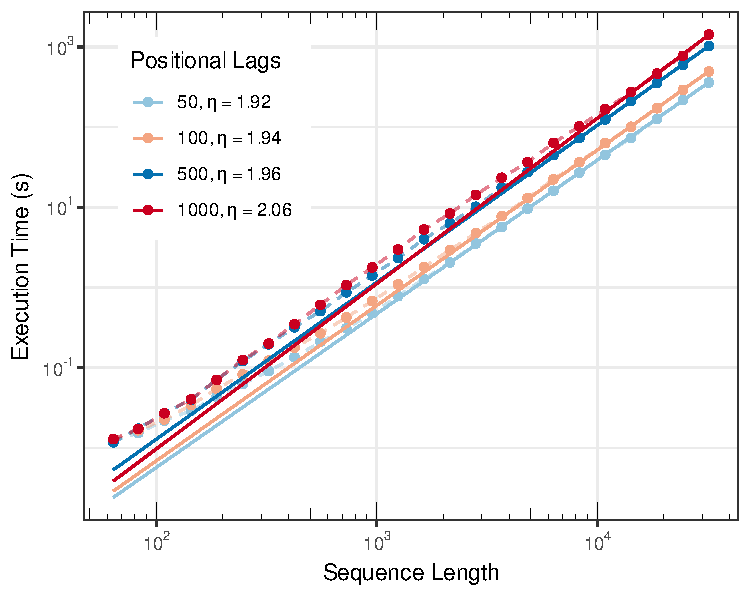
\includegraphics[width=1.0\linewidth]{../res/images/rafft/executiontime_lags-1.pdf}
				}
		}} \hfill
	\end{minipage}%
	\begin{minipage}[b]{.5\linewidth}
	\centering
	\subfloat[CPU times respect to the stack size ($N$)]{
		\label{fig:cputime_ss}{
			\scalebox{0.9}{
				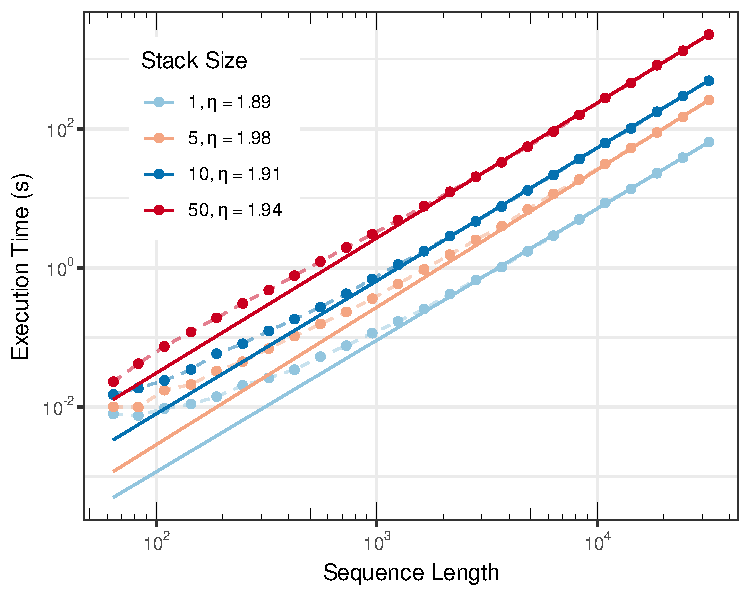
\includegraphics[width=1.0\linewidth]{../res/images/rafft/executiontimes_stack_sizes.pdf}
			}	
	}}
\end{minipage}%

	\caption{\label{Fig:scalability}\textbf{Impact of the number of positional lags $n$ and the stack size $N$ on the runtime complexity.} For a corresponding length, we generated $30$ random sequences, and averaged their execution times. Solid lines indicate the estimated time complexity $O(L^\eta)$ where $\eta$ is obtained with a non-linear regression on these average execution times for (A) Different number of positional lags $n$ and (B) Different stack sizes $N$.}
\end{figure} 

In sum, \texttt{RAFFT}'s performance shows a significant improvement compared to three folding tools (\texttt{RNAfold}, \texttt{RNAstructure}, and \texttt{ContraFold}), and we can approximate its theorical time complexity to $O(L^2\log L)$, where $L$ is the sequence length. However, its average CPU time scales with respect to the stack size and the number of positional lags considered. When $N=1$ and $n=100$, \texttt{RAFFT} CPU time is lower than all of the four tools except for sequences longer than $10^4$. But when considering $N=50$ stacks, \texttt{LinearFold} showed better performance.  Fitting the empirical CPU times of each tool to a non-linear regression showed that all the methods scaled with respect to the sequence length whereas, \texttt{LinearFold} scales linearly (i.e. $L=1$) followed by \texttt{RAFFT} with an exponent of $L\approx2$, the \ac{MFE} prediction methods scale cubically. Now, does the improvement in CPU time guarantee the quality of the predictions? The following section analyses the quality of the structure predictions.

\subsection{Accuracy of the predicted structural ensemble}

After comparing \texttt{RAFFT}'s computational time to existing tools, it is also essential to assess the quality of the predicted secondary structures. The quality of each tool's predictions is measured using two statistical metrics: the \ac{PPV} and the sensitivity. This section presents the quality comparison of \texttt{RAFFT} predictions to the four previously mentioned tools,  i.e. \texttt{RNAfold}, \texttt{RNAstructure}, \texttt{LinearFold}, \texttt{Contrafold} and the \ac{ML} method \texttt{Mxfold2}. 

We started by analyzing the prediction performances with respect to sequence lengths: we averaged the performances at fixed sequence length. \autoref{perf_fig} shows the performance in \ac{PPV} and sensitivity for the five methods. It shows that the \ac{ML} method (\texttt{Mxfold2}) consistently outperformed \texttt{RAFFT} and the other predictions. When comparing only the \ac{MFE} predictions produced using the \ac{DP} tools, \texttt{LinearFold} outperformed all other tools (\texttt{RNAfold} and \texttt{RNAstructure}) for both short and long sequences. The $t$-test between the \ac{ML} and the most used \ac{MFE} prediction tool (\texttt{RNAfold}) revealed not only a significant difference (p-value \(\approx\) $10$\textsuperscript{$-12$}) but also a substantial improvement of $14.5\%$ in \ac{PPV}. \texttt{RAFFT} showed performances similar to \texttt{RNAfold}; but, \texttt{RAFFT} is significantly less accurate ($p$-value \(\approx\) $0.0002$), with a drastic loss of performance for sequences of length greater than $300$ nucleotides (See also \autoref{Tab:average_perf}).

However, are there relevant structures in the ensemble predicted by our method? To address this question we retained the structure with the best score among the $50$ recorded structures per sequence. We obtained an average \ac{PPV} of $60.0\%$ and an average sensitivity of $62.8\%$ over all the dataset. The gain in terms of \ac{PPV}/sensitivity is especially pronounced for sequences of length $\leq 200$ nucleotides, indicating the presence of biologically more relevant structures in the predicted ensemble than the thermodynamically most stable one (\ac{PPV} was =$79.4\%$, and sensitivity=$81.2\%$). The average scores are shown in \autoref{Tab:average_perf}. We also investigated the relation to the number of bases between paired bases (base-pair spanning), but we found no striking effect, as already pointed out in one previous study \cite{amman13_troub_long_range_base_pairs_rna_foldin}.

%\begin{landscape}
\begin{table*}[htbp]
	\caption{\label{Tab:average_perf}\textbf{Average performance displayed in terms of \ac{PPV} and sensitivity.} The metrics were first averaged at fixed sequence length, limiting the over-representation of shorter sequences. The first two rows show the average performance for all the sequences for each method. The bottom two rows correspond to the performances for the sequences of length \(\leq\) $200$ nucleotides.}
	\centering
	\hspace*{-1cm}
	\begin{tabular}{lrrrrrrr}
		\hline
		& \texttt{RNAfold} & \texttt{LinearFold} & \texttt{RNAstructure}  & \texttt{CONTRAfold} & \texttt{Mxfold2} & \texttt{RAFFT} & \texttt{RAFFT}* \\
		\hline
		& \multicolumn{6}{c}{All sequences}\\
		\cmidrule{2-8}
		\ac{PPV}         & 55.9 &	60.6 &	54.7 &	58.4 &	70.4 &	47.7 & 60.0 \\
		Sensitivity & 63.3 &	58.9 &	61.5 &	65.2 &	77.1 &	52.8 & 62.8 \\
		\hline
		& \multicolumn{6}{c}{Sequences with lengths \(\leq 200\)}\\
		\cmidrule{2-8}
		\ac{PPV}         & 59.5 &	63.2 &	58.2 &	60.5 &	76.7 &	57.9 & 79.4  \\
		Sensitivity & 65.5 &	59.4 &	63.8 &	65.9 &	82.9 &	63.2 & 81.2 \\
		\hline
		
		%\hline
		%& \multicolumn{6}{c}{Sequences with lengths \(> 200\)}\\
		%\cmidrule{2-8}
		%PPV         & 48.2 &	58.4 &	51.7 &	60.5 &	76.7 &	38.7 & 43.0 \\
		%Sensitivity &56.14&	58.5 &	59.6 &	65.9 &	82.9 &	43.55 & 46.6 \\
		%\hline
	\end{tabular}
	
\end{table*}
%\end{landscape}


\begin{figure*}[t!]
	\centering
	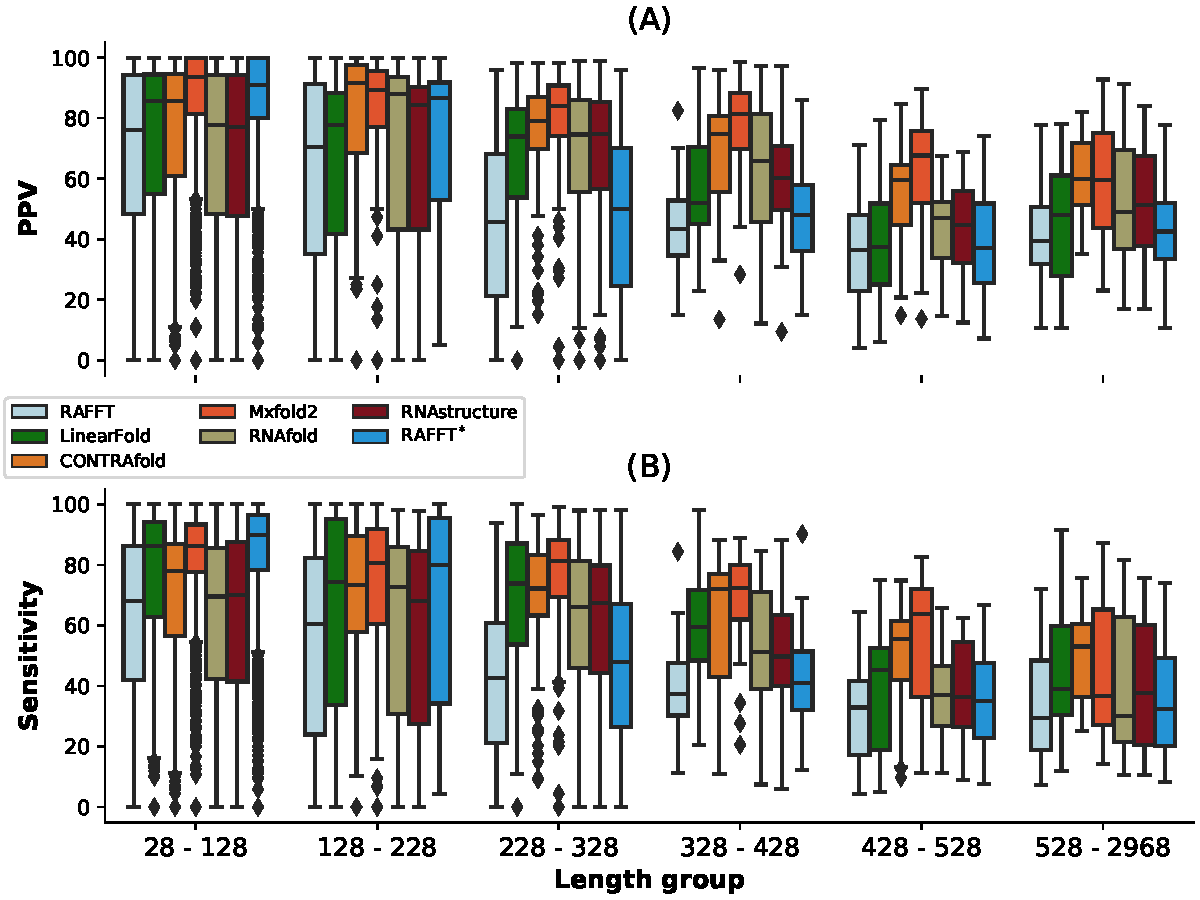
\includegraphics[width=1.\linewidth]{../res/images/rafft/accuracy.pdf}
	\caption{\label{perf_fig} \textbf{\texttt{RAFFT}'s performance on folding task.} (A) \ac{PPV} \emph{vs} sequence length. In the top panel, \texttt{RAFFT} (in light blue) shows the \ac{PPV} score distributions when for the structure (out of $N=50$ predictions) with the lowest free energy, whereas \texttt{RAFFT}* (in blue) shows the best \ac{PPV} score in that ensemble. (B) Sensitivity \emph{vs} sequence length.}
\end{figure*}

All methods performed poorly on two groups of sequences: one group of $80$ nucleotides long RNAs, and the second group of around $200$ nucleotides (three examples of such sequences are shown in the Appendix A3.1 ). Both groups have large unpaired regions, which for the first group lead to structures with average free energies $9.8\ \textrm{kcal/mol}$ according to our dataset. The \ac{PCA} analysis of the native structure space, shown in \autoref{perf_pca}, reveals a propensity for interior loops and the presence of large unpaired regions like hairpins or external loops. \autoref{perf_pca} shows the structure space produced by \texttt{Mxfold2}, which seems close to the native structure space. In contrast, the structure spaces produced by \texttt{RAFFT} and \texttt{RNAfold} are similar and more diverse.
\begin{figure}[t!]
	\centering
	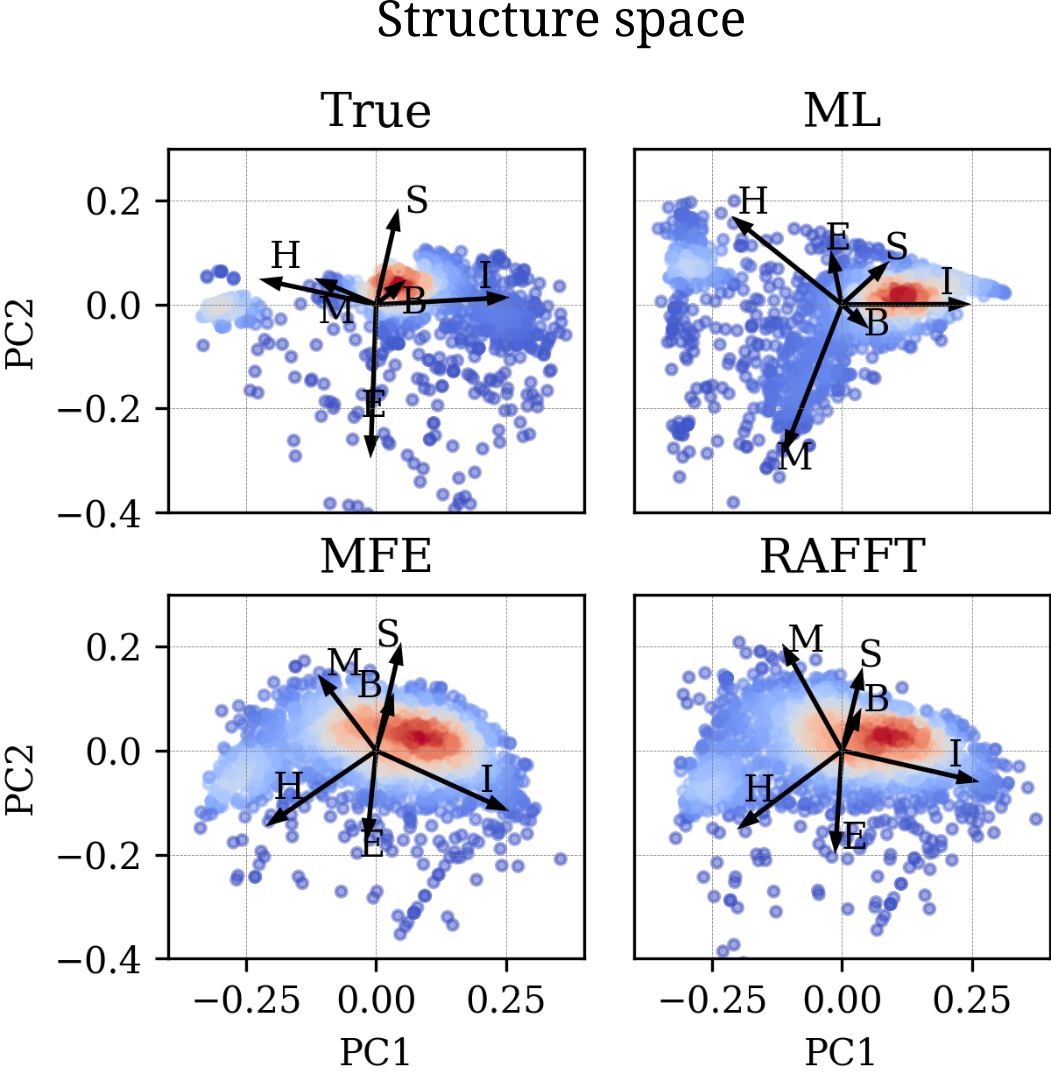
\includegraphics[width=.9\linewidth]{../res/images/rafft/perf_pca.png}
	\caption{\label{perf_pca} \textbf{Structure space analysis.} \ac{PCA} for the
		predicted structures using \texttt{RAFFT, RNAfold, MxFold2} compared to the
		known structures denoted ``True''.}
\end{figure}
\begin{figure*}[t!]
	\centering
	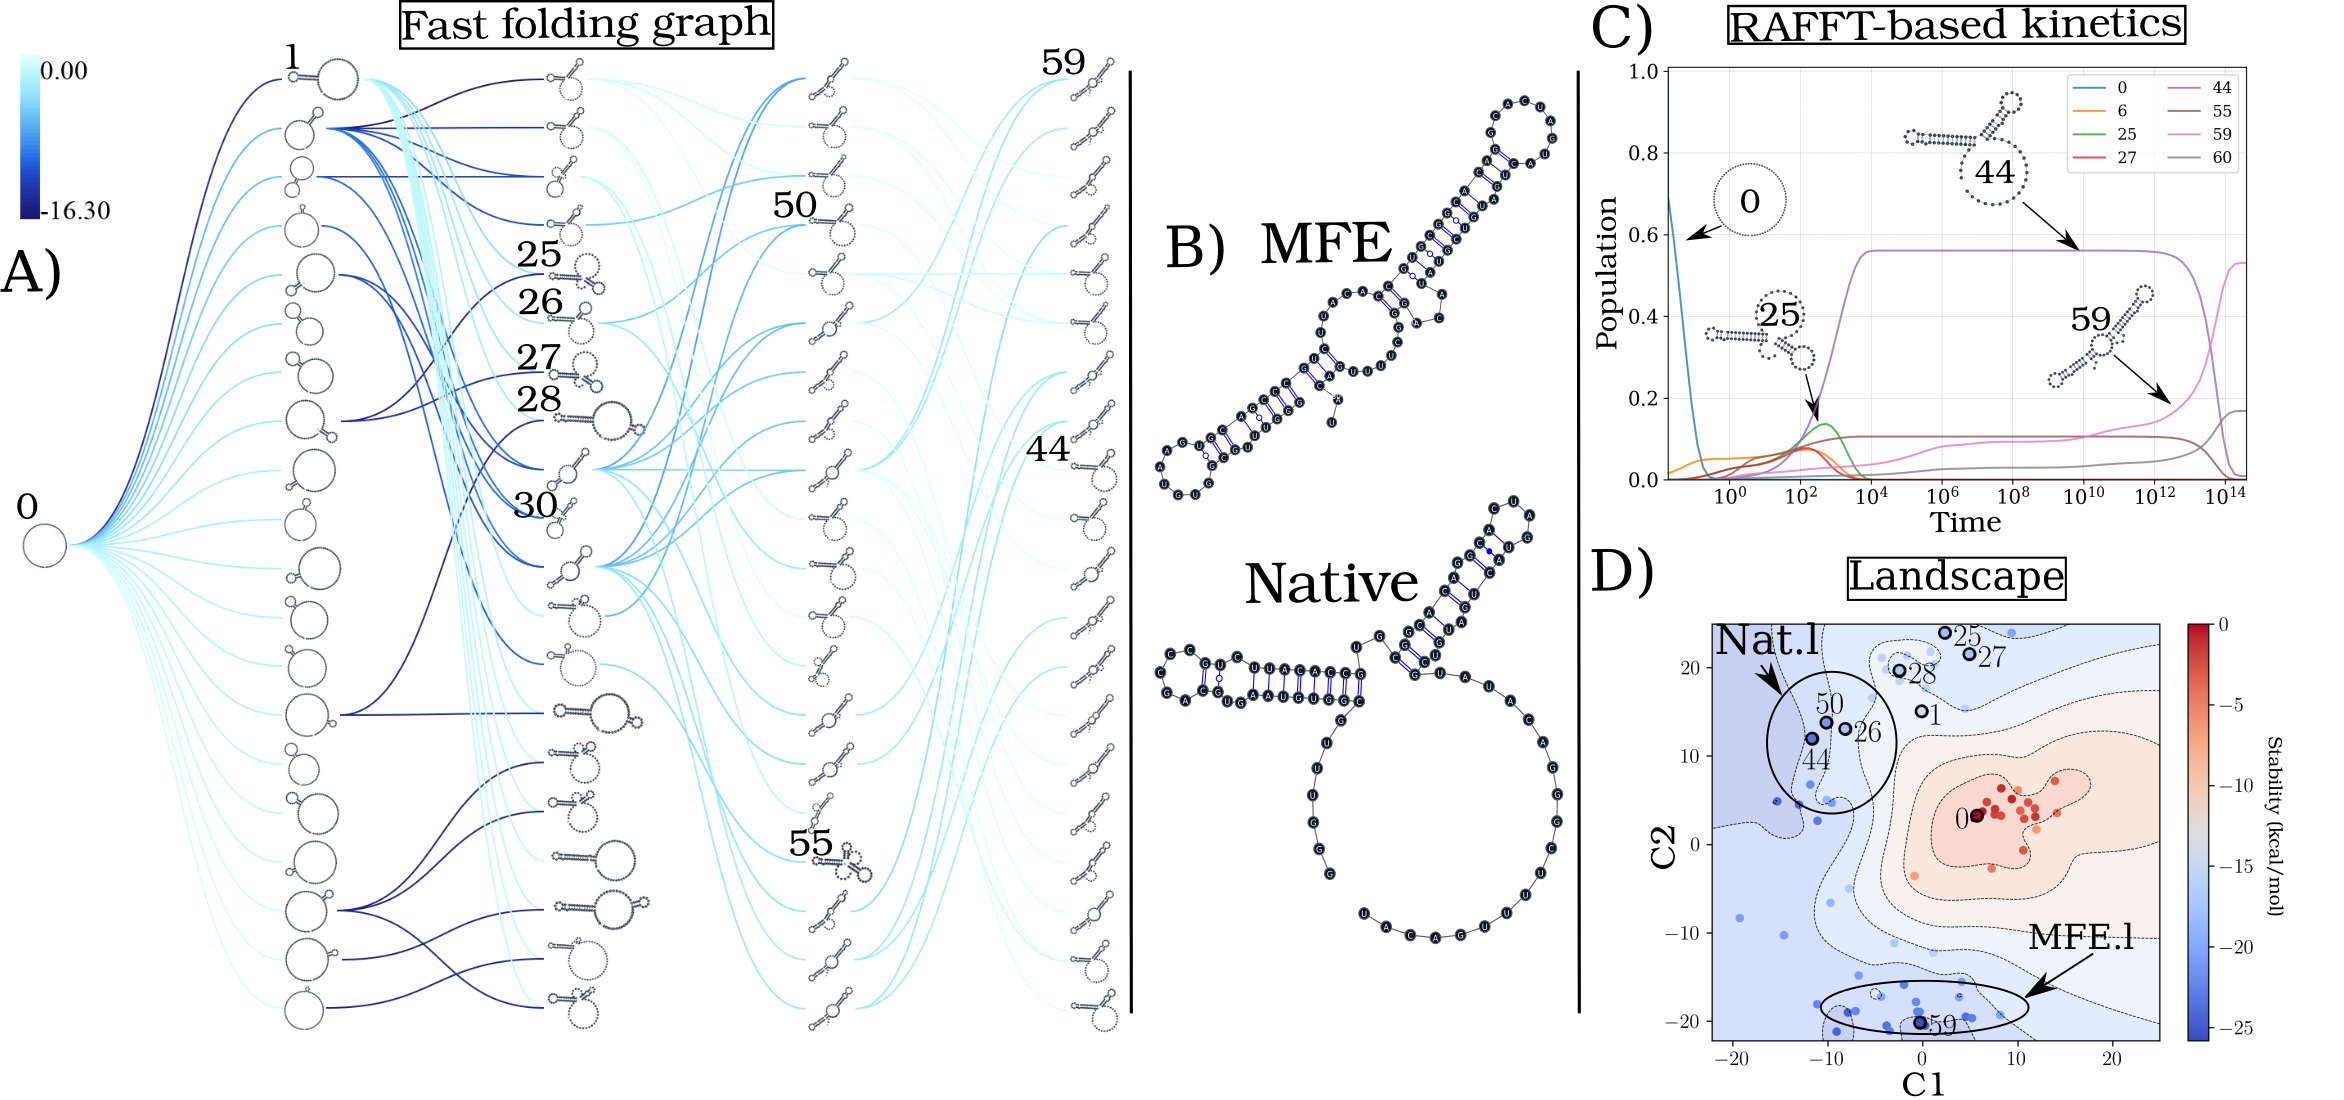
\includegraphics[width=1.\linewidth]{../res/images/rafft/test_case.png}
	\caption{\label{test_case}\textbf{Application of the folding kinetic ansatz on \ac{CFSE}.}  (A) Fast-folding graph in four steps and $N=20$ structures stored in a stack at each step. The edges are coloured according to \(\Delta \Delta G\). At each step, the structures are ordered by their free energy from top to bottom. The minimum free energy structure found is at the top left of the graph. A unique ID annotates visited structures in the kinetics. For example, ``$59$" is the ID of the \ac{MFE} structure. (B) \ac{MFE} (computed with \texttt{RNAfold}) and the native \ac{CFSE} structure. (C)The change in structure frequencies over time. The simulation starts with the whole population in the open-chain or unfolded structure (ID 0). The native structure (\textbf{Nat.l}) is trapped for a long time before the \ac{MFE} structure (\textbf{MFE.l}) takes over the population. (D) Folding landscape derived from the $68$ distinct structures predicted using \texttt{RAFFT}. The axes are the components optimized by the MDS algorithm, so the base-pair distances are mostly preserved. Observed structures are also annotated using the unique ID. \ac{MFE}-like structures (\textbf{MFE.l}) are at the bottom of the figure, while native-like (\textbf{Nat.l}) are at the top.}
\end{figure*}

In summary, we performed the prediction quality comparison for different sequence lengths. The dataset was divided into two sets: one with lengths less than $200$ nucleotides and the rest constituting the second. 
Because \texttt{RAFFT} predicts an ensemble of structures, which contrasts the other tools, we also distinguish the single prediction (\texttt{RAFFT}) comparison from the ensemble one (\texttt{RAFFT}*). Overall, on average, \texttt{RAFFT} performed qualitatively poorer than existing tools in terms of both \ac{PPV} and sensitivity. The \ac{ML} method, \texttt{Mxfold2} outperformed all existing methods for different \ac{RNA} sequence lengths but equalized \texttt{RAFFT}* performance  for sequences of length less than $200$ nucleotides. The later showed that \texttt{RAFFT} predicted ensemble contains sequences of biological interest. We further assess the quality of that ensemble with the proposed kinetics ansatz. The next section discusses two \ac{RNA} kinetic test cases: the application of the kinetic ansatz on \ac{CFSE} and a bistable \ac{RNA} sequence. 
\subsection{Applications to the RNA kinetics}

Furthermore, the ensemble of structures predicted by \texttt{RAFFT} is analyzed using a kinetics ansatz to extract information about the dynamic of RNA folding. This section analyses the kinetics of two \ac{RNA} sequences using \texttt{RAFFT} predicted pathways.

We started with the \ac{CFSE}, a natural \ac{RNA} sequence of $82$ nucleotides with a structure determined by sequence analysis and obtained from the RFAM database. This structure has a pseudoknot which is not taken into account here.

\autoref{test_case}A and \autoref{test_case}B show respectively the fast-folding graph constructed using \texttt{RAFFT}, and the \ac{MFE} and native structures for the \ac{CFSE}. The fast-folding graph is computed in four steps. At each step, stems are constructed by searching for $n=100$ positional lags and, a set of $N=20$ structures (selected according to their free energies) are stored in a stack. The resulting fast-folding graph consists of $68$ distinct structures, each of which is labelled by a number. Among the structures in the graph, $6$ were found similar to the native structure ($16/19$ base-pairs differences). The structure labelled ``$29$'' in the graph leading to the \ac{MFE} structure ``$59$'' is the $9^{th}$ in the second stack. When storing less than $9$ structures in the stack at each step, we cannot obtain the \ac{MFE} structure using \texttt{RAFFT}; this is a direct consequence of the greediness of the proposed method. To visualize the energy landscape drawn by \texttt{RAFFT}, we arranged the structures in the fast-folding graph onto a surface according to their base-pair distances; for this we used the multidimensional scaling algorithm implemented in the \texttt{scipy} package.  \autoref{test_case}D shows the landscape interpolated with all the structures found; this landscape illustrates the bi-stability of the \ac{CFSE}, where the native and \ac{MFE} structures are in distinct regions of the structure space.

From the fast-folding graph produced using \texttt{RAFFT}, the transition rates from one structure in the graph to another are computed using the formula given in \autoref{Eq:metropolis}. Starting from a population of unfolded structure and using the computed transition rates, the native of structures is calculated using \autoref{Eq:kenetics}. \autoref{test_case}C shows the frequency of each structure; as the frequency of the unfolded structure decreases to $0$, the frequency of other structures increases. Gradually, the structure labelled ``$44$", which represents the \ac{CFSE} native structure, takes over the population and gets trapped for a long time, before the \ac{MFE} structure (labelled "$59$") eventually becomes dominant. Even though the fast-folding graph does not allow computing energy landscape properties (saddle, basin, etc.), the kinetics built on it reveals a high barrier separating the two meta-stable structures (\ac{MFE} and native). 

\begin{figure*}[t!]
	\centering
	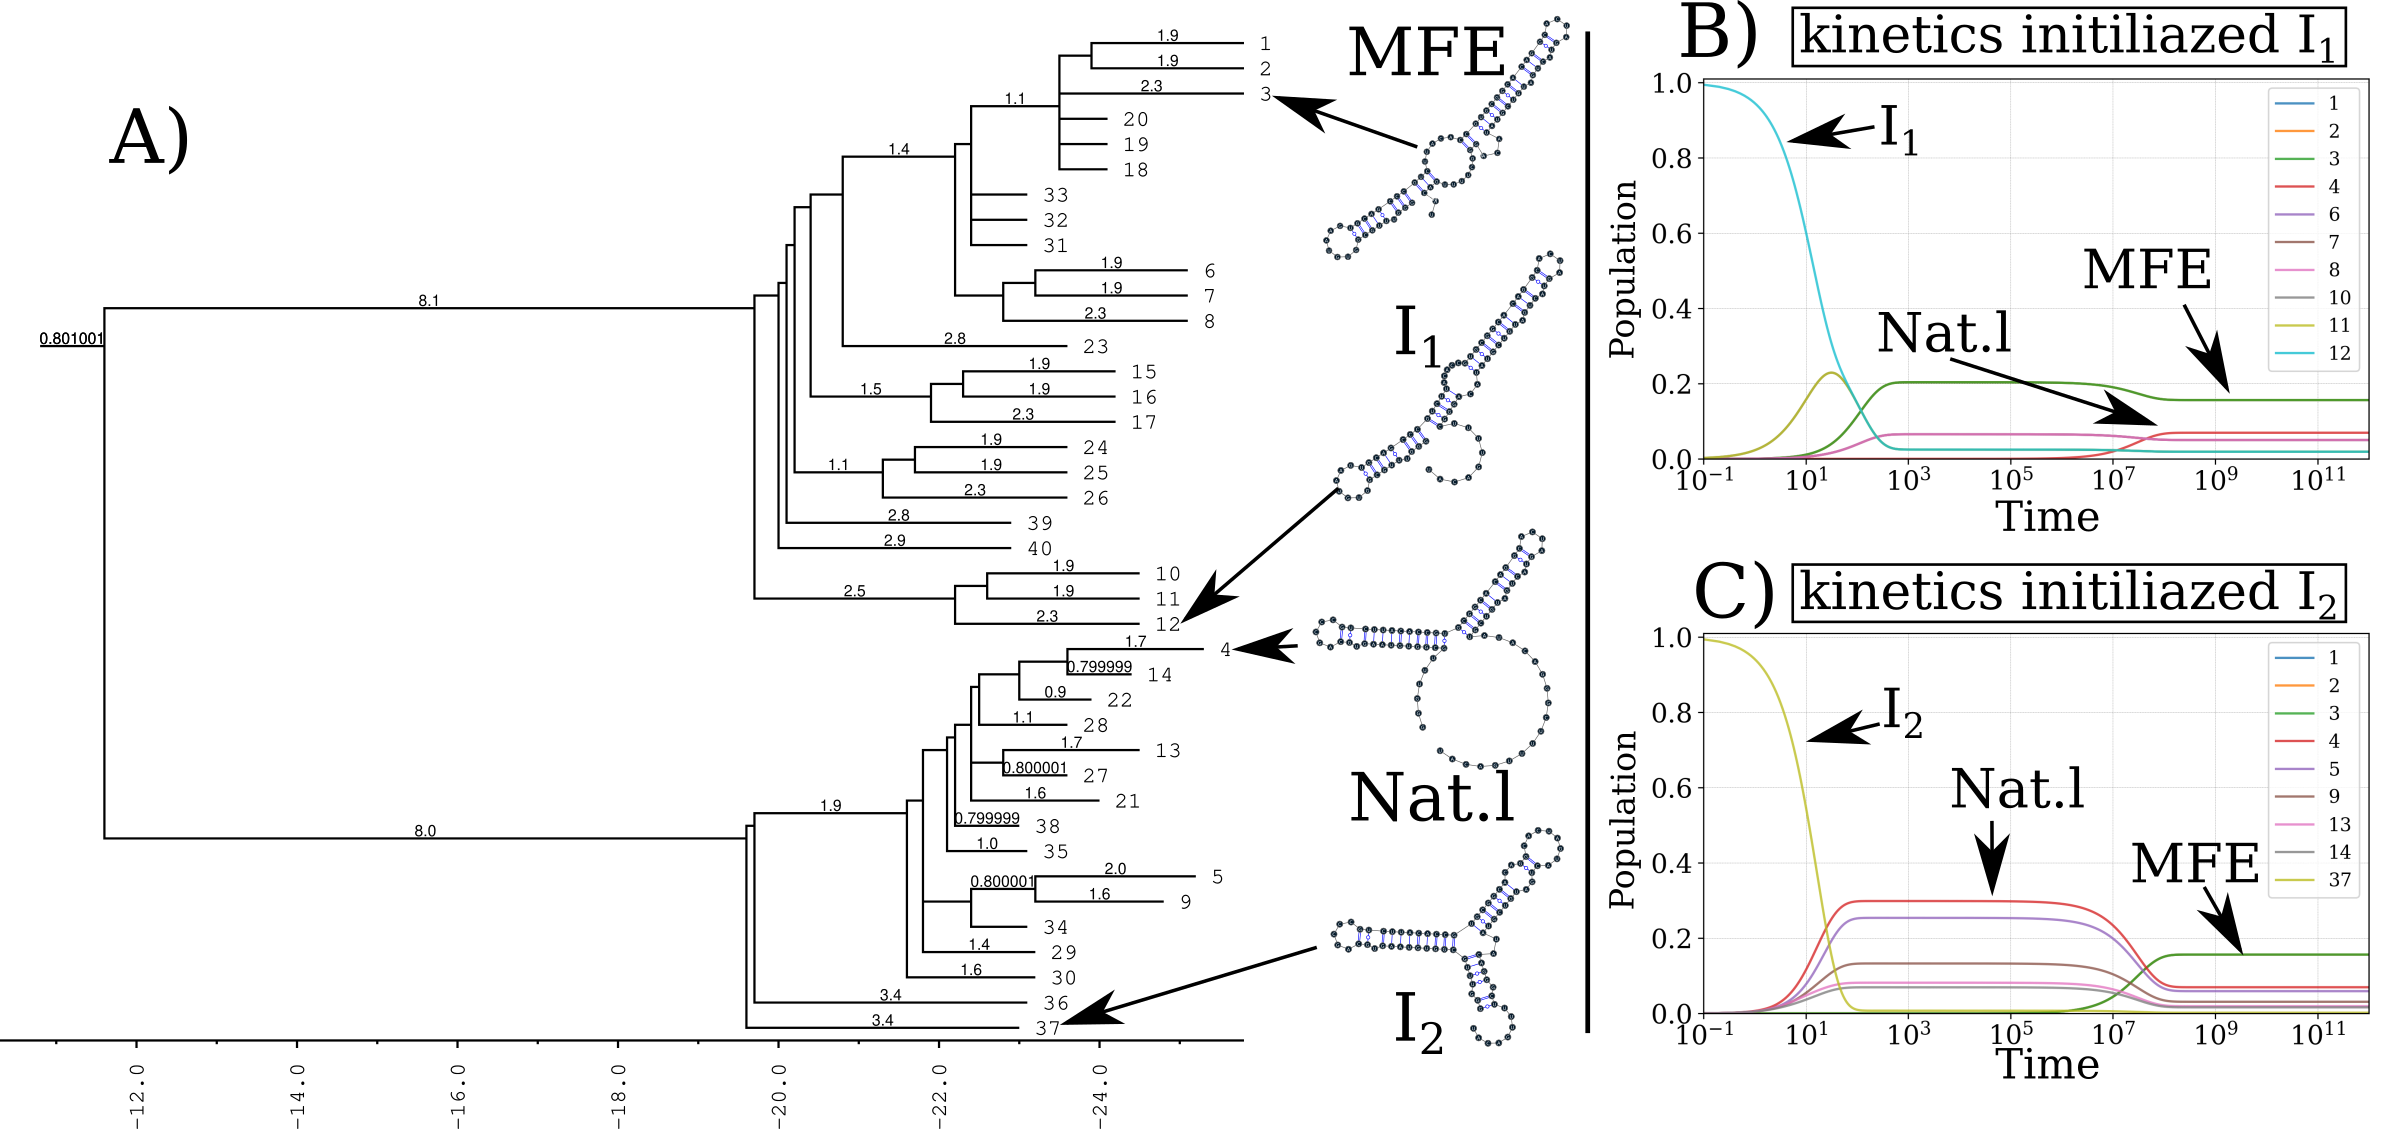
\includegraphics[width=0.9\linewidth]{../res/images/rafft/kinetic_treekin.png}
	\caption{\label{treekin}\textbf{Folding kinetics of \ac{CFSE} using \texttt{Treekin}. }A) Barrier tree of the \ac{CFSE}. From a set of $1.5\times10^6$ sub-optimal structures, $40$ local minima were found,  connected through saddle points. The tree shows two alternative structures separated by a high barrier with the global minimum (\ac{MFE} structure) on the right side. (B) Folding kinetics with initial population $I_1$. Starting from an initial population of $I_1$, as the initial frequency  decreases, the others increase, and gradually the \ac{MFE} structure is the only one populated.  (C) Folding kinetics with initial population $I_2$. When starting with a population of $I_2$, the native structure (labelled \textbf{Nat.1} ) is observable, and gets kinetically trapped for a long time due to the high energy barrier separating it from the \ac{MFE} structure.}
\end{figure*}

\begin{figure*}[t]
	\centering
	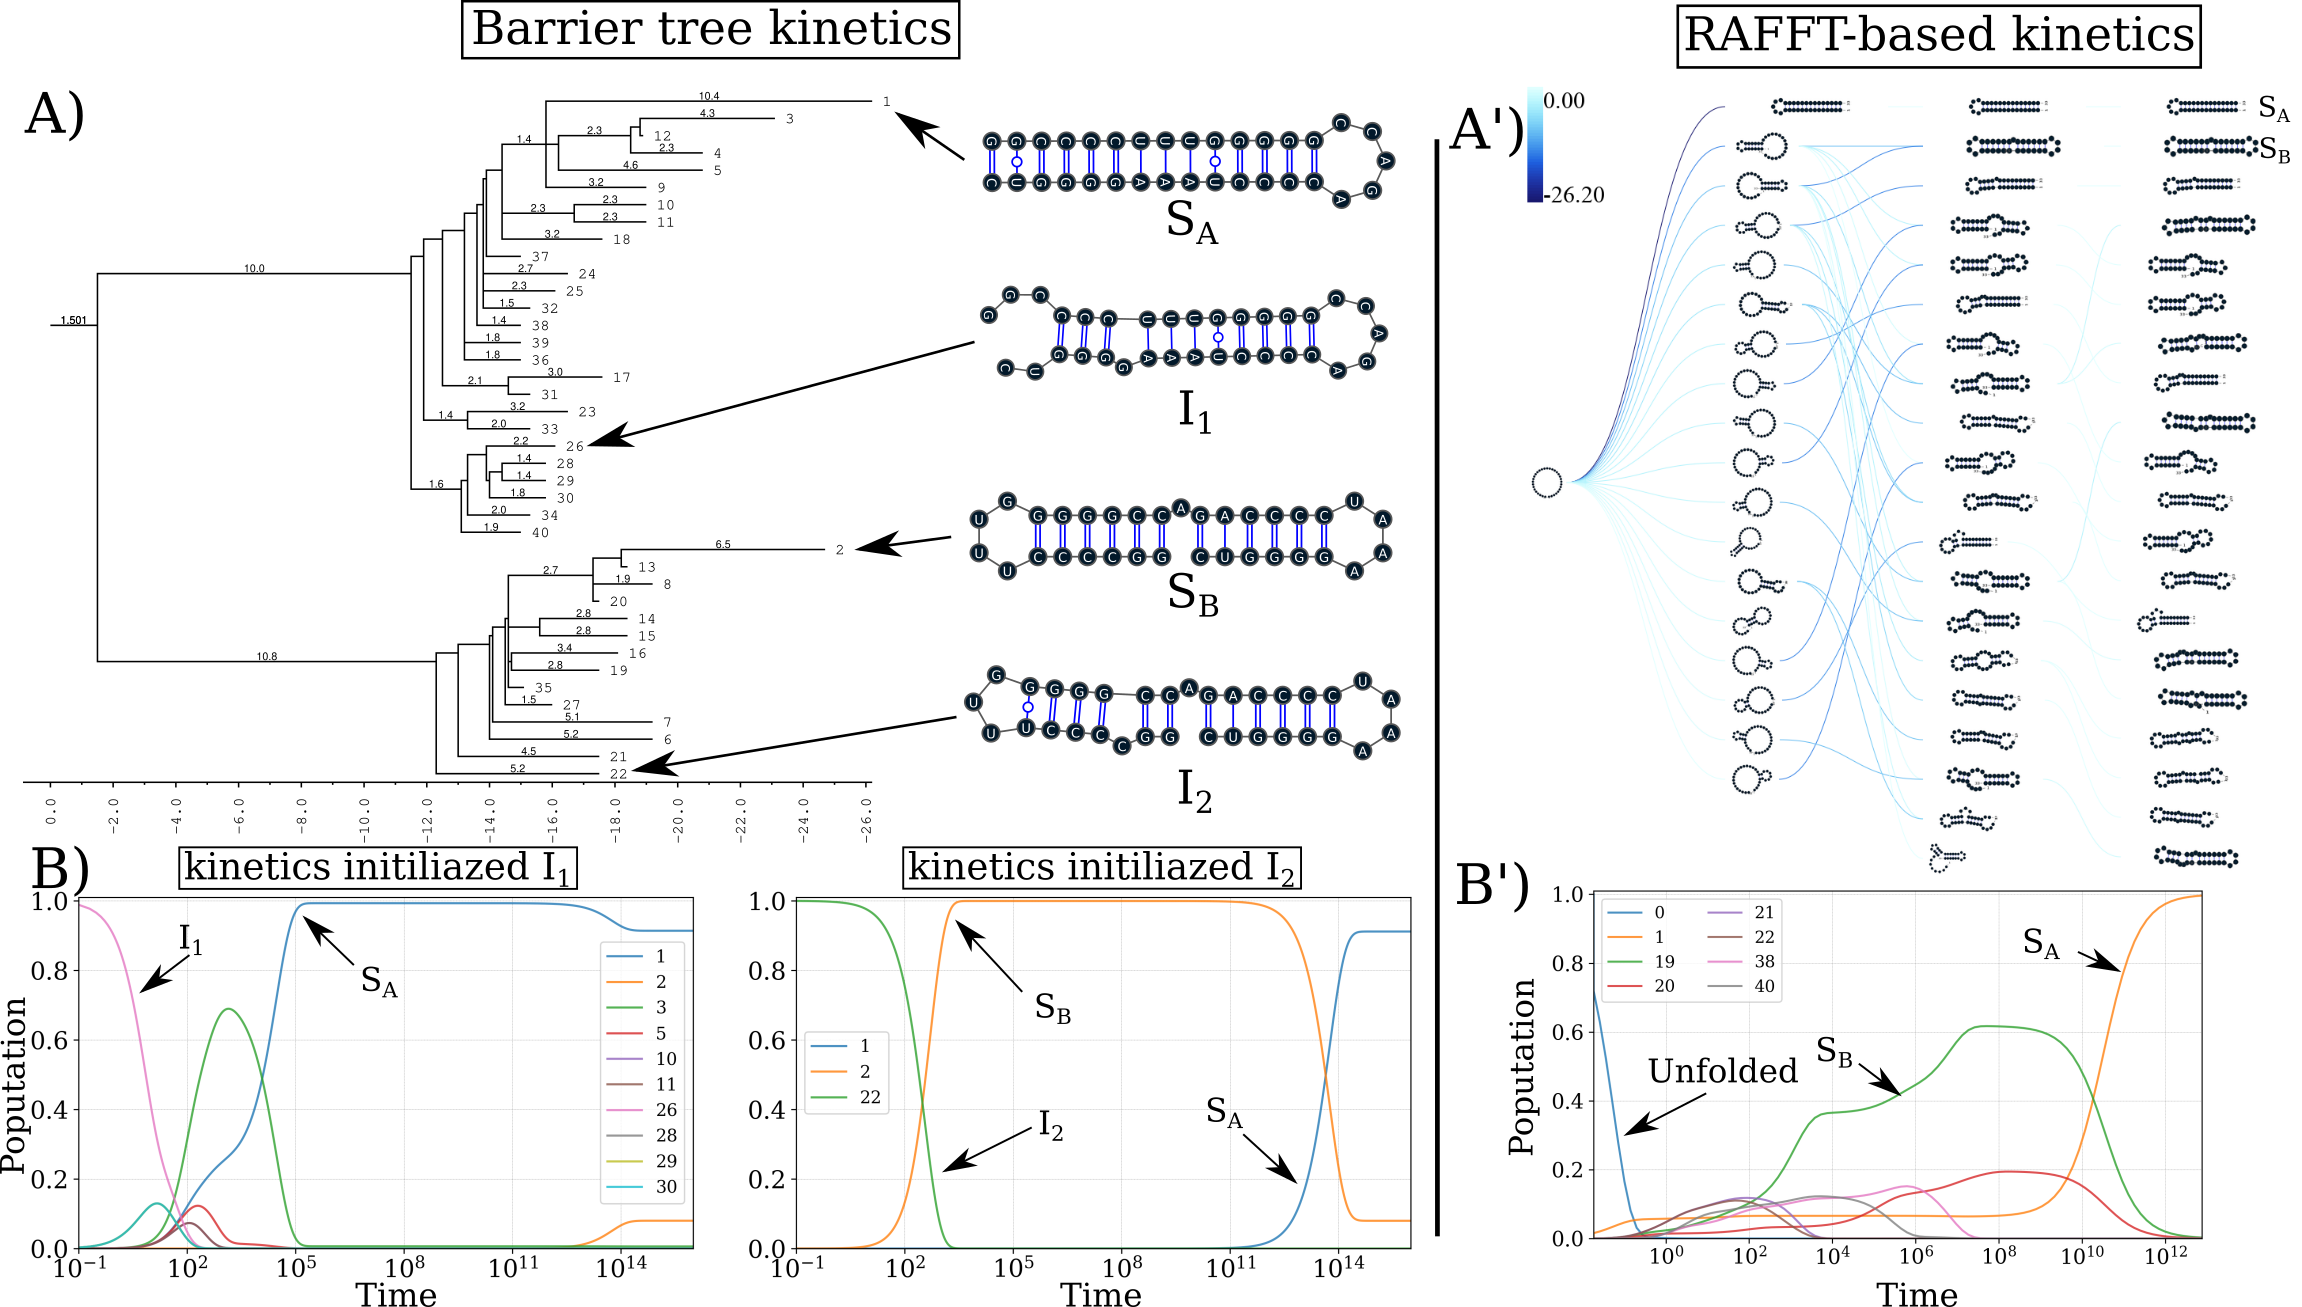
\includegraphics[width=0.9\linewidth]{../res/images/rafft/kine_bi_sta.png}
	\caption{\label{class_examp}\textbf{\texttt{RAFFT} \emph{vs} \texttt{Treekin}: folding kinetics of a bi-stable \ac{RNA} sequence.} (A) Barrier tree for the bi-stable example sequence. The local minima and the corresponding barriers are computed from the complete enumeration of the structure space. The bi-stability is visible on the barrier tree through the two branches separated by a high barrier.  (B) Folding kinetics trajectories. The left plot shows the folding dynamics starting from a population with $I_1$, and the right size is the kinetics when the population is initialized in structure $I_2$. When starting from $I_1$, $S_A$ is quickly populated; starting from $I_2$, the bi-stability is more apparent.  (A') Fast-folding graph using \texttt{RAFFT}. A maximum of $N=20$ structures are stored in a stack at each step and overall $46$ distinct structures are visited. (B') Folding kinetics trajectory obtained from the fast-folding graph (indices are different from the barrier tree indices). The dynamics starts with a population with only unfolded structure, and slowly, $S_B$ is populated and gets trapped for a long time before the \ac{MFE} structure $S_A$ becomes populated.}
\end{figure*}
Our kinetic simulation was then compared to \texttt{Treekin} \cite{flamm02_barrier_trees_degen_lands}. First, we generated \(1.5 \times 10^6\) sub-optimal structures up to $15 \ \textrm{kcal/mol}$ above the \ac{MFE} structure using \texttt{RNAsubopt} \cite{lorenz11_vienn_packag}. Since the \ac{MFE} is $\Delta G_s=-25.8 \ \textrm{kcal/mol}$, the unfolded structure could not be sampled. Second, the ensemble of structures is coarse-grained into $40$ competing basins using the tool \texttt{barriers} \cite{flamm02_barrier_trees_degen_lands}, with the connectivity between basins represented as a barrier tree (see \autoref{treekin}A). When using \texttt{Treekin}, the choice of the initial population is not straightforward. Therefore we resorted to two initial structures $I_1$ and $I_2$ (see \autoref{treekin}B and \ref{treekin}C, respectively). In \autoref{treekin}B, the trajectories show that only the kinetics initialized in the structure $I_2$ can capture the complete folding dynamics of \ac{CFSE}, in which the two metastable structures are visible. Thus, in order to produce a folding kinetics in which the native and the \ac{MFE} structures are visible, the kinetic simulation performed using \texttt{Treekin} required a particular initial condition and a barrier tree representation of the energy landscape built from a set of  $1.5 \times 10^6$ structures. By contrast, using the fast-folding graph produced by \texttt{RAFFT}, which consists only of $68$ distinct structures, our kinetic simulation produces complete folding dynamics starting from a population of unfolded structure.

As a second illustrative example, we applied both kinetic models to the classic bi-stable sequence. For \texttt{Treekin}, we first sampled the whole space of \(20 \times 10^3\) sub-optimal structures from the unfolded state to the \ac{MFE} structure, and from that set, $40$ basins were also computed using \texttt{barriers}. The barrier tree in \autoref{class_examp} shows the bi-stable landscape, where the two deepest minima are denoted $S_A$ and $S_B$. As in the first application, we also chose two initializations with the structures denoted $I_1$ and $I_2$ in \autoref{class_examp}A and \ref{class_examp}B. Secondly, we simulate the kinetics starting from the two initial conditions (See \autoref{class_examp}B). When starting from $I_2$, the slow-folding dynamics is visible:  $S_B$ first gets kinetically trapped, and the \ac{MFE} structure ($S_A$) only takes over later on. For our kinetic ansatz, we started by constructing the fast-folding graph using \texttt{RAFFT}, consisting of only $46$ distinct structures. The resulting kinetics, shown in \autoref{class_examp}B' was found qualitatively close to the barrier kinetics initialized with structure $I_2$. Once again, with few as $48$ structures, our proposed kinetic ansatz can produce complete folding dynamics starting from a population of unfolded structure.

In both examples, our kinetic ansatz derived from the fast folding graph predicted by \texttt{RAFFT} produces complete folding kinetic trajectories, using fewer structures than the existing methods that required the complete enumeration of the fitness landscape (i.e. all structures and their associated energies). Despite the poor validation procedure of our kinetic ansatz, we believe that the \ac{RNA} pathways predicted by \texttt{RAFFT} could contain structures of biological pertinence. An analysis of the sample structures produced by \texttt{RAFFT} is provided in Appendix \autoref{app:sec:kinetic} and a discussion on some limitations in \autoref{ch:limitations}.

\section{Conclusion}
We have proposed a method for \ac{RNA} structure, and dynamics predictions called \texttt{RAFFT}. Our method is inspired by the experimental observation of parallel fast-folding pathways. To mimic this observation, we designed an algorithm that produces parallel folding pathways in which stems are formed sequentially. Taking advantage of the \ac{FFT}, the time complexity of our method was slowed down to $O(L^2\log L)$, thus improving the cubic time complexity of classic \ac{DP} methods. Then, we proposed a kinetic ansatz that exploits the parallel fast-folding pathways predicted to model how different conformations are populated over time. Our kinetic ansatz produced complete folding dynamics without sampling the entire conformation space. However, our method also presents some limitations that will be discussed in \autoref{ch:conclusion}.
